\documentclass[11pt]{article}
\usepackage{amsmath,amssymb,booktabs,graphicx,geometry,bm}
\geometry{margin=1in}
\newcommand{\R}{\mathrm{R}}
\newcommand{\Ext}{\mathrm{E}}
\newcommand{\Exp}{\mathbb{E}}
\newcommand{\ind}{\mathbb{1}}
\title{\vspace{-2em}Safe selective borrowing of external controls\\ via covariate-shift-adjusted longitudinal residual-rank screening}
\author{}
\date{}

\begin{document}
\maketitle
\vspace{-3em}

\begin{abstract}
\noindent Hybrid controlled trials can borrow external controls (ECs) for precision, but naive full borrowing is catastrophically biased when some ECs are incompatible. We rank each EC's longitudinal residual nonconformity score among the randomized controls---weighted to absorb baseline covariate shift---and borrow only the conforming ECs through a transported AIPW. Three design choices make it work: (i)~\emph{symmetric} two-sided trimming, which keeps the borrowed control mean unbiased; (ii)~\emph{cross-validated} (CV+) rank calibration, which does not waste the scarce randomized-control sample; and (iii)~an \emph{estimand-matched} score. In simulation the method is unbiased, controls type-I error, and beats RCT-only on RMSE and power while approaching the oracle screen; it is robust to working-model misspecification and to covariate shift; and it avoids the bias/type-I traps of the one-sided screen and the max score. The contribution is \emph{safe, valid, robust} borrowing---not a large efficiency gain.
\end{abstract}

\section{The problem, and the idea}
A randomized trial has few controls; a registry or historical arm offers many external controls that could sharpen the treatment-effect estimate. Borrowing \emph{all} of them is dangerous: if a subset is incompatible (a hidden shift in the control outcome), the borrowed control mean is biased and coverage collapses (the ``Full EC-AIPW'' row of Table~\ref{tab:ref} below: bias $-0.42$, type-I $0.42$). RCT-only is always valid but discards the external information.

The idea is \emph{selective} borrowing: keep the compatible ECs, drop the rest, and do so from the outcomes themselves rather than a propensity heuristic. For each EC we compute a longitudinal residual score, rank it among the randomized-control scores (a conformal $p$-value), and keep those that look like ordinary randomized controls. Two extensions beyond ordinary conformal selective borrowing are essential here and are our methodological contribution: \emph{covariate-shift weighting} of the rank (randomized and external covariate distributions differ), and an \emph{estimand-aware longitudinal} score integrated with a refitted external-control AIPW.

\begin{figure}[t]\centering
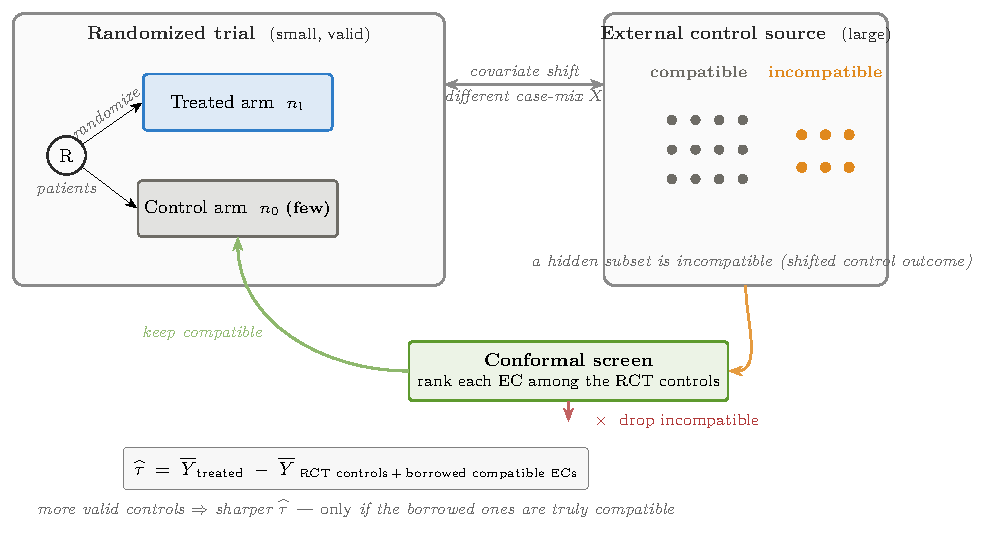
\includegraphics[width=\linewidth]{fig_design.pdf}
\caption{The setup. A small randomized trial compares a treated and a control arm; a large external source offers extra controls, but a hidden subset is incompatible and the two sources differ in baseline case-mix (covariate shift). We screen each external control by how it ranks against the randomized controls, borrow the compatible ones into the control comparison, and drop the rest---sharpening $\widehat\tau$ only with controls that are truly exchangeable.}
\label{fig:design}
\end{figure}

\section{Method}
Let $S{=}1$ index the trial and $S{=}0$ the external source; within the trial $A{=}1{/}0$ is randomized treatment/control. Screening compares randomized controls ($S{=}1,A{=}0$) to external controls ($S{=}0$). For a subject with baseline covariates $X$ and visit trajectory $\bm Y$, fit a working control-mean model $\widehat m(X)$ on the randomized controls, form the residual $\bm r=\bm Y-\widehat m(X)$, and reduce it to a scalar nonconformity score $V=s(\bm r)$ aligned with the estimand contrast $Z=c^\top\bm Y$ (visit-average, last-minus-baseline, or Mahalanobis).

\begin{figure}[t]\centering
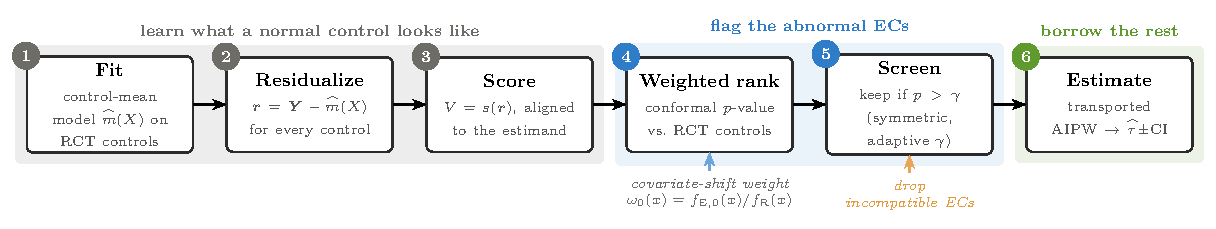
\includegraphics[width=\linewidth]{fig_pipeline.pdf}
\caption{The method in six steps. Steps 1--3 learn what an ordinary randomized control looks like (fit a control-mean model, residualize, reduce to an estimand-aligned score); steps 4--5 rank each external control against the randomized controls---reweighted for covariate shift---and keep only the conforming ones; step 6 refits a transported AIPW on the randomized controls plus the retained external controls.}
\label{fig:pipeline}
\end{figure}

\paragraph{The weighted conformal screen.} With $\omega_0(x)=f_{\Ext,0}(x)/f_\R(x)$ the compatible-EC-to-RCT density ratio, the upper-tail weighted $p$-value of an external score $V^{\Ext}_j$ against the randomized-control calibration scores $\{V^\R_i\}$ is
\[
\widehat p^{\,w}_j=\frac{\omega_0(X_j)+\sum_i \omega_0(X_i)\,\ind\{V^\R_i\ge V^{\Ext}_j\}}{\omega_0(X_j)+\sum_i \omega_0(X_i)},
\]
and we retain $\{j:\widehat p^{\,w}_j>\gamma\}$. Weighting makes the randomized-control score distribution represent what a \emph{compatible} EC would show under its own covariate mix, so the ranks are calibrated despite covariate shift.

\paragraph{Estimator.} On the retained ECs we refit the source density, outcome model, and inverse-variance borrowing weight and form the transported AIPW control mean $\widehat\mu_{0,\gamma}^{\Ext}$, combined with the randomized-control mean as $\widehat\tau=\widehat\mu_1-\{(1-\lambda)\widehat\mu_{0}^{\R}+\lambda\,\widehat\mu_{0,\gamma}^{\Ext}\}$.

\paragraph{Three design choices that make it work.}
\begin{enumerate}\itemsep2pt
\item[(i)] \textbf{Symmetric two-sided trimming.} Screen on $|V|$ with a single threshold, trimming both tails equally. This keeps the retained conditional mean unmoved, so the borrowed control mean stays \emph{unbiased}. The one-sided (non-symmetric) alternative cuts only the high tail; it detects directional contamination harder but truncates the clean upper tail and biases the estimate---its apparent power is a bias/type-I artifact (Table~\ref{tab:ref}).
\item[(ii)] \textbf{CV+ rank calibration.} Cross-fit the score across folds instead of a one-time train/calibrate split, so the entire (scarce) randomized-control sample calibrates the ranks. This is the main efficiency lever (Table~\ref{tab:robust}).
\item[(iii)] \textbf{Adaptive, de-biased threshold.} Choose $\gamma$ per dataset to minimize a label-free estimated MSE (squared distance to the no-borrow estimate, de-biased by the paired bootstrap variance, plus bootstrap variance), following the CSB principle.
\end{enumerate}

\begin{figure}[t]\centering
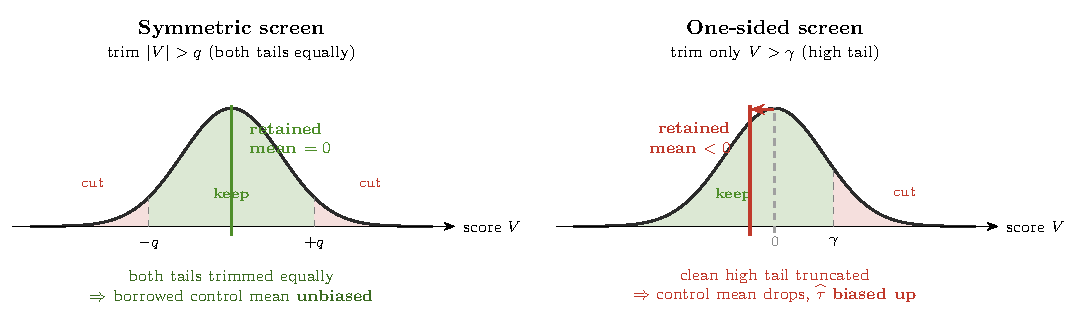
\includegraphics[width=0.95\linewidth]{fig_trimming.pdf}
\caption{Why the screen is \emph{symmetric} (design choice~(i)). Trimming both tails of the clean, roughly symmetric score equally leaves the retained mean at $0$, so the borrowed control mean stays unbiased (left). Cutting only the high tail---the one-sided screen that chases directional contamination---truncates the clean upper tail, pulls the retained mean down, and biases $\widehat\tau$ upward (right); its extra ``power'' is that bias, not signal.}
\label{fig:trimming}
\end{figure}

\section{Why screen on the score, not the outcome (Figure~\ref{fig:mech})}
Figure~\ref{fig:mech} shows one simulated draw at the reference-cell setup ($\Delta{=}8$). On the raw outcome (top) the compatible ECs (blue) overlap the randomized controls (gray) but sit slightly higher \emph{purely because the external mix carries more severe subjects}---covariate shift, not incompatibility---while the contaminated ECs (amber) sit far right; a raw-outcome threshold would confound the two. Ranking each EC's covariate-adjusted score against the randomized controls converts it to a conformal $p$-value (bottom): contaminated ECs pile near $0$ and fall below the threshold $\gamma$ (dropped), while compatible ECs are roughly uniform and kept. The screen truncates this calibrated $p$-value scale at $\gamma$, not the raw outcome; because the underlying score is trimmed symmetrically, the retained control mean stays unbiased.

\begin{figure}[ht]\centering
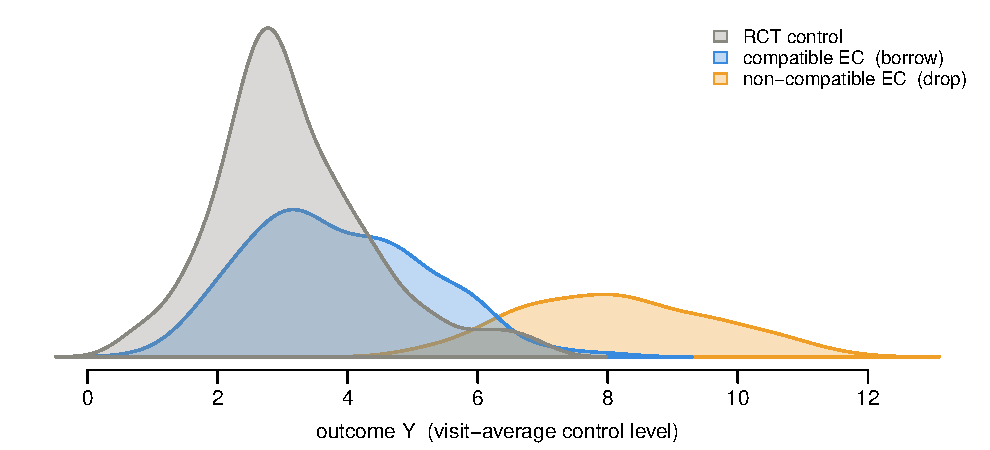
\includegraphics[width=.92\linewidth]{fig_outcome.pdf}\\[2pt]
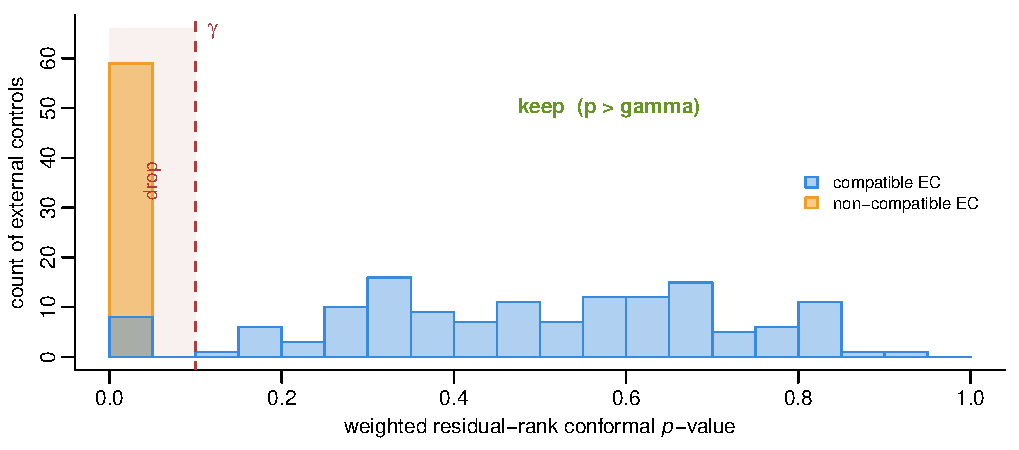
\includegraphics[width=.92\linewidth]{fig_pval.pdf}
\caption{Outcome density (top) and weighted residual-rank conformal $p$-values (bottom) for randomized controls, compatible ECs (borrowed), and non-compatible ECs (dropped); reference-cell setup ($\Delta{=}8$, CV+). The raw outcome confounds covariate shift with contamination; the $p$-value scale separates them---contaminated ECs pile below $\gamma$, compatible ECs spread uniformly---and the screen keeps those with $p>\gamma$.}
\label{fig:mech}
\end{figure}

\section{The method beats RCT-only on all four criteria (Table~\ref{tab:ref})}
Table~\ref{tab:ref} is a head-to-head at one reference cell (base binary DGP, contamination fraction $\pi_B{=}0.3$, a detectable signal-to-noise level, visit-average estimand). The symmetric adaptive screen (\textbf{sym-ada}) is the only \emph{attainable} method that beats RCT-only on all four criteria at once---unbiased, lower RMSE, controlled type-I, higher power---reaching most of the way to the (unattainable) oracle screen. The non-symmetric screens buy more raw power only by paying bias and inflated type-I, so that power is not valid inference. Naive full borrowing is catastrophic.

\begin{table}[ht]\centering
\caption{Reference cell (base binary DGP, $\pi_B{=}0.3$, pattern~A, $\Delta{=}8$, visit-average estimand, $\tau{=}0.4625$; weighted CV+ rank calibration, correct model; $300$ replicates, $B{=}500$ bootstraps). sym-ada beats RCT-only on all four criteria at once (unbiased; RMSE $0.18$ vs.\ $0.20$; type-I no worse than RCT-only, $0.06$; power $0.73$ vs.\ $0.64$), approaching the oracle. The non-symmetric screens' higher power is a bias/type-I artifact; full borrowing is catastrophic.}
\label{tab:ref}
\begin{tabular}{lcccccc}
\toprule
Method & Detection & False-excl. & Bias & RMSE & Type-I & Power \\
\midrule
RCT-only            & --- & --- & $-0.00$ & $0.20$ & $0.06$ & $0.64$ \\
Full EC-AIPW        & --- & --- & $-0.42$ & $0.49$ & $0.42$ & $0.06$ \\
Oracle              & $1.00$ & $0.00$ & $-0.00$ & $0.17$ & $0.06$ & $0.75$ \\
\midrule
\textbf{sym-ada (default)} & $1.00$ & $0.10$ & $0.00$ & $\mathbf{0.18}$ & $0.06$ & $\mathbf{0.73}$ \\
nonsym-ada          & $0.99$ & $0.07$ & $+0.05$ & $0.20$ & $0.08$ & $0.84$ \\
nonsym-fix          & $1.00$ & $0.32$ & $+0.31$ & $0.36$ & $0.31$ & $0.99$ \\
\bottomrule
\end{tabular}
\end{table}

\section{Robustness, and the score must match the drift (Table~\ref{tab:robust})}
Moving one axis at a time off the sym-ada/CV+ baseline (Table~\ref{tab:robust}):
\begin{itemize}\itemsep1pt
\item \textbf{Model misspecification: robust.} Even dropping the covariate from the working mean model barely changes anything---the model error is shared by randomized and compatible controls and absorbed by the randomized-control calibration.
\item \textbf{Covariate-shift weighting: a low-cost safeguard.} Under the correct model the standardized residual is covariate-free, so weighting is a no-op; it earns its keep under misspecification and low signal-to-noise (dropping it then raises false-exclusion).
\item \textbf{CV+ over split.} Cross-fitting the calibration lifts power by $\sim$$0.06$ ($0.65$ to $0.71$ here) and widens the RMSE gain, at controlled type-I, by not wasting the randomized controls.
\item \textbf{Score shape must match the drift shape.} For a ramp drift the visit-average score sees only half the signal and loses to RCT-only; the Mahalanobis (quadratic) score recovers detection and a real power gain; the max score is a type-I trap (high power via bias and inflated type-I) and should not be used.
\end{itemize}

\begin{table}[ht]\centering
\caption{One-axis robustness off the sym-ada/CV+ baseline (hetero base DGP, $\pi_B{=}0.3$, $\Delta{=}8$; $300$ replicates, $B{=}500$). Each row changes one thing.}
\label{tab:robust}
\begin{tabular}{lcccccc}
\toprule
Setting & Bias & RMSE & Type-I & Power & Detection & False-excl. \\
\midrule
baseline (sym-ada, CV+) & $-0.00$ & $0.18$ & $0.04$ & $0.71$ & $0.99$ & $0.10$ \\
severe model misspec.\  & $+0.00$ & $0.19$ & $0.04$ & $0.70$ & $1.00$ & $0.11$ \\
unweighted (correct)    & $-0.00$ & $0.18$ & $0.05$ & $0.71$ & $1.00$ & $0.09$ \\
split instead of CV+    & $-0.00$ & $0.19$ & $0.05$ & $0.65$ & $0.99$ & $0.11$ \\
C-slope drift, $c_2$    & $-0.02$ & $0.19$ & $0.05$ & $0.63$ & $0.88$ & $0.14$ \\
C-slope drift, Mahalanobis & $-0.01$ & $0.19$ & $0.04$ & $0.68$ & $0.95$ & $0.17$ \\
C-slope drift, max (trap)  & $+0.04$ & $0.21$ & $0.13$ & $0.79$ & $0.87$ & $0.06$ \\
\bottomrule
\end{tabular}
\end{table}

\section{Scope, limits, and positioning}
The efficiency upside is real but bounded: even the oracle screen lowers RMSE by only $\sim$15--25\%, because the treated arm is not borrowable, so the borrowable share of the estimator's variance is $n_{\R,1}/(n_{\R,0}+n_{\R,1})$. Borrowing therefore helps most when the randomized controls are scarce---the realistic hybrid-trial regime---but the screen also needs enough randomized controls to calibrate; CV+ widens this window. The score must be chosen for the anticipated drift shape. Deeper validation on a covariate-driven (plasmode) design is the natural next step.

The right framing is \textbf{insurance, not a free lunch}: selective conformal borrowing turns naive full borrowing's catastrophic bias into \emph{valid, robust} inference that deletes incompatible external controls and delivers a modest, real efficiency gain when the randomized arm is underpowered---with a clear mechanistic account of \emph{why} (symmetric trimming for unbiasedness, screening on the covariate-adjusted score, and cross-fit calibration).

\begin{thebibliography}{9}\small
\bibitem{zhu} K.~Zhu et al. Conformal selective borrowing for external controls. \emph{ICML}, 2025.
\bibitem{tib} R.~Tibshirani et al. Conformal prediction under covariate shift. \emph{NeurIPS}, 2019.
\bibitem{jin} Y.~Jin, E.~Cand\`es. Weighted conformal prediction. 2026.
\bibitem{zhou} Zhou et al. Causal estimators for incorporating external controls in randomized trials with longitudinal outcomes. \emph{JRSS-A}, 2025.
\end{thebibliography}
\end{document}
